\documentclass{article}
\usepackage{lmodern}
\usepackage{graphicx}
\usepackage[utf8]{inputenc}
\usepackage[T1]{fontenc}
\usepackage{enumitem}
\usepackage[cache=false,outputdir=build]{minted}
\usepackage{amsmath, amsfonts, amssymb, amsthm}
\usepackage{float}
\usepackage{hyperref}
\usepackage[hypcap=false]{caption}
\usepackage{tikz,xcolor}
\usepackage{appendix}
\usepackage{tabularx}

%\usepackage[framed,numbered,autolinebreaks,useliterate]{mcode}
%\usepackage{lstlisting}

\usepackage{multicol}
\usepackage{xcolor, colortbl}
\usepackage{xfrac}
% Margins
\usepackage[top=2.5cm, left=3cm, right=3cm, bottom=4.0cm]{geometry}
\usepackage{changepage}
\usepackage{textgreek}
\usepackage{physics}
\usepackage{gensymb} %Provides generic commands for \degree, \celsius...
\usepackage{cancel}
\usepackage{mathtools}
\usepackage{subcaption}
\usepackage{parskip}



\begin{document}

%%%%%%%%%%%%%%%%%%%%%%%%%%%%%%% FRONT PAGE %%%%%%%%%%%%%%%%%%%%%%%%%%%%%%%

\newcommand{\HRule}{\rule{\linewidth}{0.5mm}} % Defines a new command for the horizontal lines, change thickness here

\begin{center}
    \vspace*{0.5 cm}

\begin{figure}[!ht]
\centering
   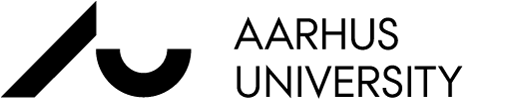
\includegraphics[width=130mm]{Photos/aulogo.png}
\end{figure}    
\vspace{2.5cm}

\textsc{\Large MSc in Mechanical Engineering, 3rd Semester}\\[0.7 cm]
   
\rule{\linewidth}{0.5 mm} \\[0.3 cm]
{ \Huge \bfseries Assignment 2}\\
{\rule{\linewidth}{0.5 mm}} \\[1 cm]
	
\textsc{\LARGE Finite Element Method}\\[0.35 cm]
    
\vspace{.4cm}    

\center 
\Large
\emph{\textbf{Instructors:}} \\
Lili Zhang\\
Mikkel Melters Pedersen\\
\vspace{0.5cm}

\center 
\Large
\emph{\textbf{Teaching Assistants:}} \\
Lasse Buus Jacobsen\\
Mathias Sätherström Boye\\
\vspace{1cm}  

\center
\emph{\textbf{Student:}}\\ % Nöfn á höfundum skýrslu
Kristofer Bjarmi Schram \\
202102204\\

\vspace{1cm}
 
\textbf{\large 14. October 2022}

\vfill % Fill the rest of the page with whitespace
\end{center}
\newpage


%%%%%%%%%%%%%%%%%%%%%%%%%%%%%%% Problems %%%%%%%%%%%%%%%%%%%%%%%%%%%%%%%

\section*{Rectangular isoparametric element}
A rectangular isoparametric with 6 nodes is shown in physical and reference space in Figure 1. It has quadratic top and bottom sides, but the vertical sides are linear. 

The element is fully constrained in nodes 5 and 6, and loaded by force two force couples in the remaining nodes. The loading corresponds to pure bending. The load magnitude is 
\vspace{0.3cm}
\[\abs{F} = 100 \, \text{N}\]
\\
The element is in a state of plane stress and exhibits linearly elastic and isotropic material behavior with properties 
\vspace{0.3cm}
\[t = 1 \, \text{mm,} \quad E = 1500 \, \text{MPa,} \quad \nu = 0.3\]
\begin{figure}[H]
    \centering
    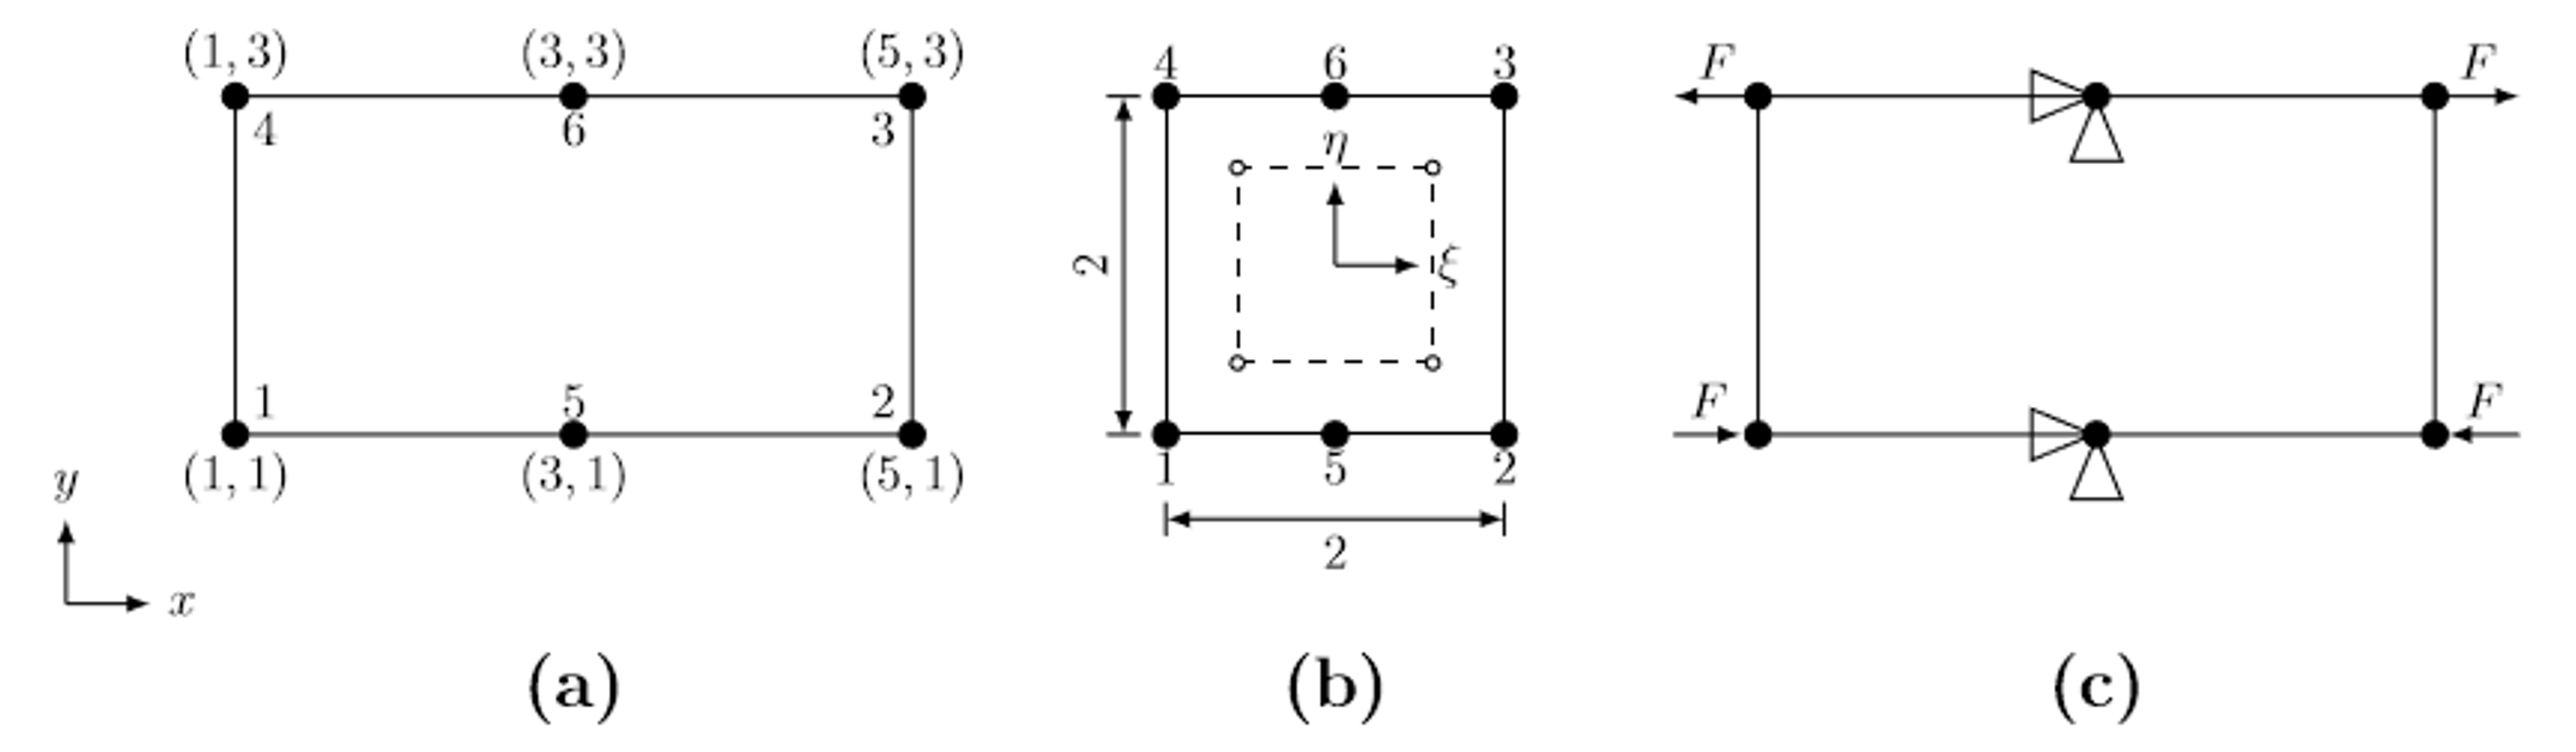
\includegraphics[width=0.8\textwidth]{Photos/ProbFig.png}
    \caption{(a) Physical element, (b) reference element \& (c) boundary conditions.}
    \label{fig:P1}
\end{figure}
\begin{enumerate}
	\item (\hyperref[code1]{Code, lines 20-40}) Using  $[\boldsymbol{X}]=\begin{bmatrix}1 & \xi & \eta & \xi\eta & \xi^2 & \xi^2\eta\end{bmatrix}$ as a recipe for the shape function values $N_{unit}$, i.e., the matrix that multiplied with the generalized coordinates $a_i$ gives the nodal coordinates $x_i$. The first column is a vector filled with 'ones'. The second and third columns are the reference coordinates $\xi$ and $\eta$ of each node. See figure 1a above. The last the three columns are calculated according to  $[\boldsymbol{X}]$. As an example, the first row would be $\begin{bmatrix}1 & \xi_1 & \eta_1 & \xi_1\eta_1 & \xi_1^2 & \xi_1^2\eta_1\end{bmatrix} = \begin{bmatrix}1 & -1 & 1 & -1 & 1 & 1\end{bmatrix}$. The full matrix is now: 

	\[N_{unit} = 
	\begin{bmatrix}
		1 & -1 & -1 & 1 & 1 & -1\\
		1 & 1 & -1 & -1 & 1 & -1\\
		1 & 1 & 1 & 1 & 1 & 1\\
		1 & -1 & 1 & -1 & 1 & 1\\
		1 & 0 & -1 & 0 & 0 & 0\\
		1 & 0 & 1 & 0 & 0 & 0
	\end{bmatrix}
	.\] 	

	The shape function matrix is now, $[N] = [\boldsymbol{X}] N_{unit}^{-1}$, (Cook, 6.1-2). 
	\[N = \begin{bmatrix}1 & \xi & \eta & \xi\eta & \xi^2 & \xi^2\eta\end{bmatrix}
	\begin{bmatrix}
		1 & -1 & -1 & 1 & 1 & -1\\
		1 & 1 & -1 & -1 & 1 & -1\\
		1 & 1 & 1 & 1 & 1 & 1\\
		1 & -1 & 1 & -1 & 1 & 1\\
		1 & 0 & -1 & 0 & 0 & 0\\
		1 & 0 & 1 & 0 & 0 & 0
	\end{bmatrix}^{-1}
	= \begin{bmatrix}N_1 & N_2 & N_3 & N_4 & N_5 & N_6 \end{bmatrix}, 
	\]
	Where, 
	\begin{align*}
		N_1 &= 
		- \frac{\eta \xi^{2}}{4} + \frac{\eta \xi}{4} + \frac{\xi^{2}}{4} - \frac{\xi}{4} &
		N_2 &= 
		- \frac{\eta \xi^{2}}{4} - \frac{\eta \xi}{4} + \frac{\xi^{2}}{4} + \frac{\xi}{4} &
		N_3 &= 
\frac{\eta \xi^{2}}{4} + \frac{\eta \xi}{4} + \frac{\xi^{2}}{4} + \frac{\xi}{4} \\
		N_4 &= 
		\frac{\eta \xi^{2}}{4} - \frac{\eta \xi}{4} + \frac{\xi^{2}}{4} - \frac{\xi}{4} &
		N_5 &= 
		\frac{\eta \xi^{2}}{2} - \frac{\eta}{2} - \frac{\xi^{2}}{2} + \frac{1}{2} &
		N_6 &= 
- \frac{\eta \xi^{2}}{2} + \frac{\eta}{2} - \frac{\xi^{2}}{2} + \frac{1}{2}
	\end{align*}

	Plotting the 1st and 5th shape function yields: 
	\begin{figure}[H]
		\centering
		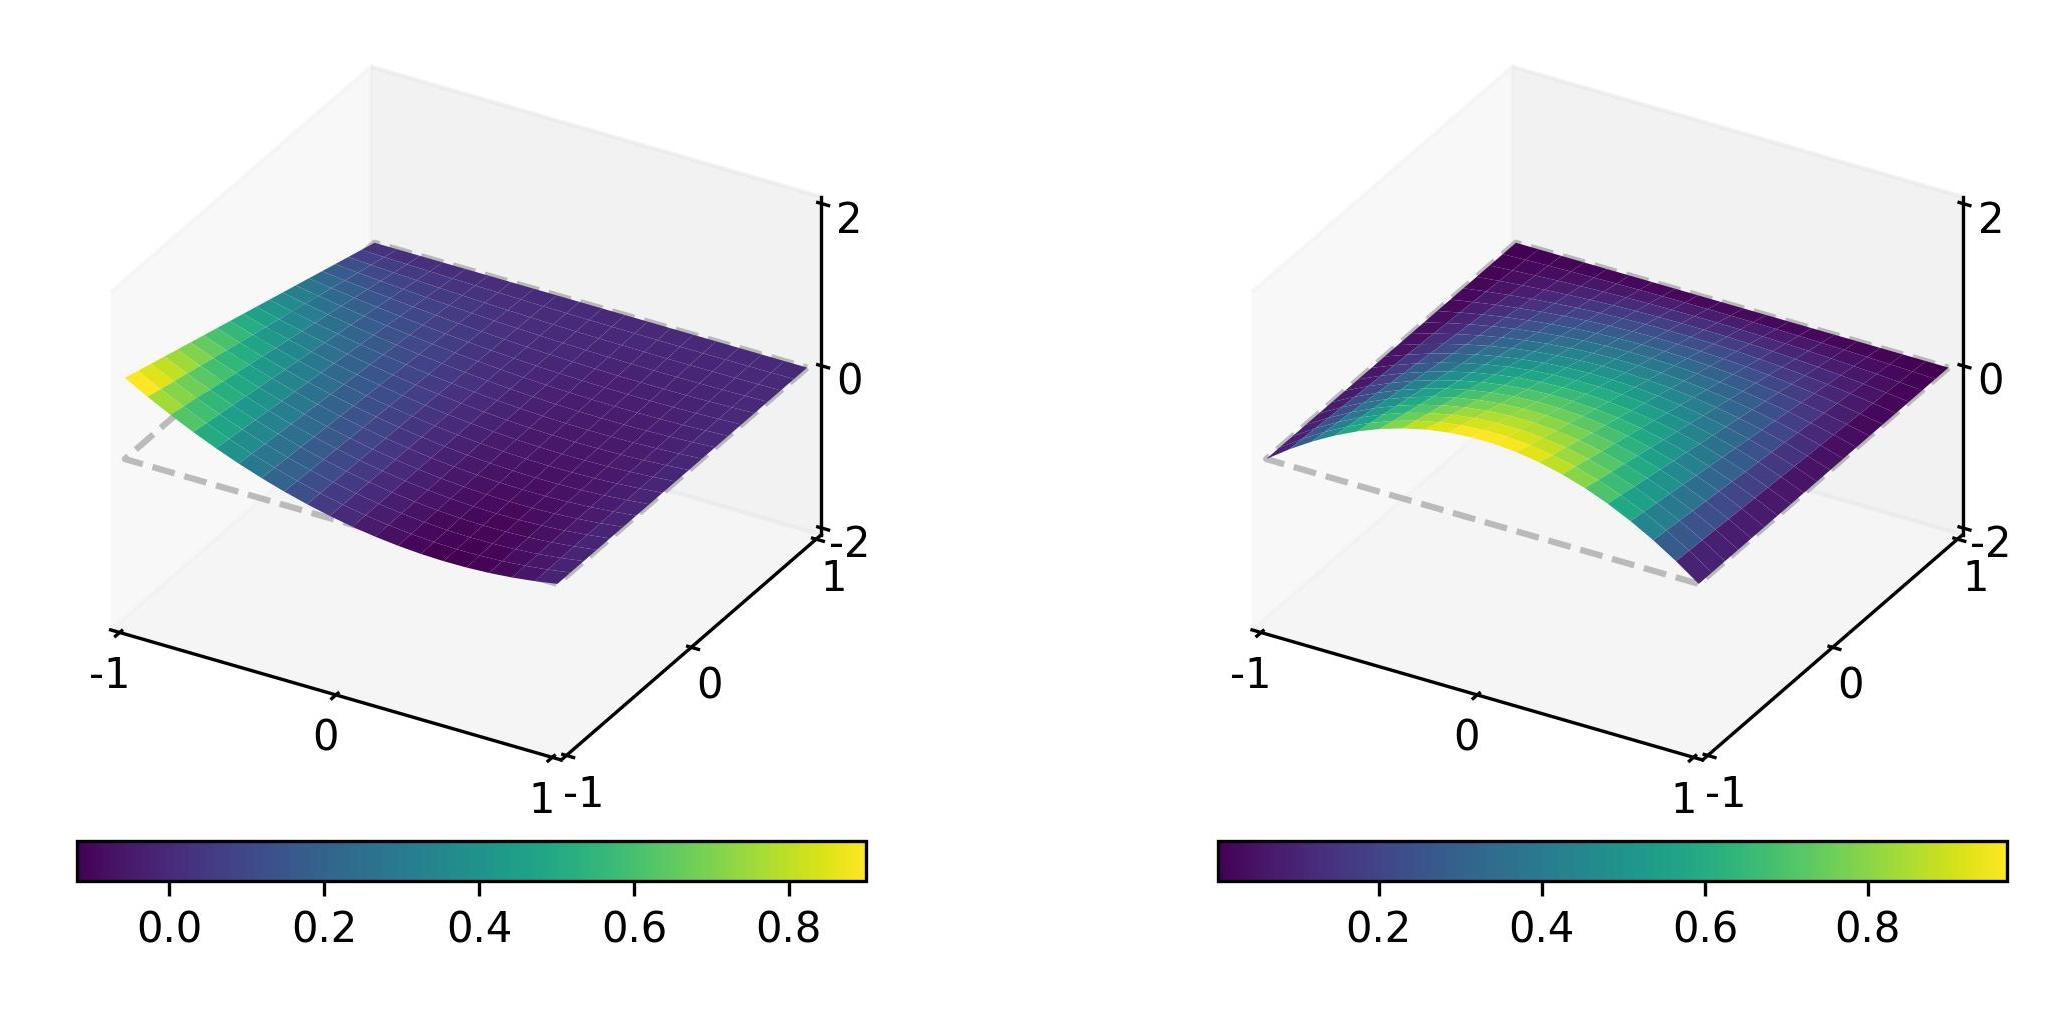
\includegraphics[width=0.8\textwidth]{Photos/N1N5.jpg}
		\caption{The 1st (left) and 5th (right) shape functions.}
		\label{fig:N1N5}
	\end{figure}

	This $[X]$ vector simply reflects the fact that two sides of the element are linear and the other quadratic. These are sometimes called transition elements and are used to connect cubic elements to quadratic. For a more common quadratic element, the  vector would be $[X] = \begin{bmatrix}1 & \xi & \eta & \xi\eta & \xi^2 & \xi^2\eta & \xi^2\eta^2 & \xi\eta^2 & \eta^2\end{bmatrix}$.

When choosing an x-vextor, the values must be balanced in both direction, which this clear ins't as there is no $\eta^2$ present. 

\item  (\hyperref[code1]{Code, lines 99-103}) The Jacobian matrix is calculated as (see \textit{Cook, 6.2-5}),

	 \[
		 [\textbf{J}] = 
		 \begin{bmatrix}
			 \sum N_{i,\xi}x_i & \sum N_{i,\xi}y_i \\
			 \sum N_{i,\eta}x_i & \sum N_{i,\eta}y_i
		 \end{bmatrix}
	,\] 

	and can be expanded, in mm, to, 
\begin{align} 
	[\mathbf{J}] = 
	\begin{bmatrix}
		N_{1,\xi} & \cdots & N_{6,\xi} \\
		N_{1,\eta} & \cdots & N_{6,\eta} 
	\end{bmatrix}
	\begin{bmatrix}
		x_1 & y_1 \\
		x_2 & y_2 \\
		x_3 & y_3 \\
		x_4 & y_4 \\
		x_5 & y_5 \\
		x_6 & y_6 
	\end{bmatrix} = 
	\begin{bmatrix}
		N_{1,\xi} & \cdots & N_{6,\xi} \\
		N_{1,\eta} & \cdots & N_{6,\eta} 
	\end{bmatrix}
	\begin{bmatrix}
		1 & 1 \\
		5 & 1 \\
		5 & 3 \\
		1 & 3 \\
		3 & 1 \\
		3 & 3 
	\end{bmatrix} = 
	\begin{bmatrix}
		2 & 0 \\
		0 & 1
	\end{bmatrix}
	\label{eq:jac}
.\end{align} 

The partial derivative in (\ref{eq:jac}) of the shape functions can be obtain by utilizing the \texttt{jacobian} function in most CAS-software. This creates a new matrix where the first row is the partial derivative of $[N]$ w.r.t. $\xi$, and the second row $[N]$ w.r.t. $\eta$. 

The determinant of the Jacobian matrix is now, 
\[
	J = \text{det}[\mathbf{J}] = \mathbf{J}_{11}\mathbf{J}_{22}-\mathbf{J}_{21}\mathbf{J}_{12} = 2
.\]

The Jacobian matrix describes the change in size of the element, due to mapping from physical system, ($x, y$) to the refrence system ($\xi, \eta$).  The individual values are the relative changes from a general coordinate in the physical system to a coordinate in the reference system, see eq. (\ref{eq:jac2}) below. 
\begin{align}
	[\mathbf{J}] = 
\begin{bmatrix}
	\frac{\partial x}{\partial \xi} & \frac{\partial x}{\partial \eta} \\
	\frac{\partial y}{\partial \xi} & \frac{\partial y}{\partial \eta} 
\end{bmatrix}
\label{eq:jac2}
\end{align}

With this, the changing area can now be described with the determinant, i.e., 
\begin{align}
	dxdy = \text{det}[\mathbf{J}]d\xi d\eta = Jd\xi d\eta
	\label{eq:jac3}
\end{align}
\item (\hyperref[code1]{Code, lines 109-126}) By utilizing the equations 6.2-9, 6.2-10 and 6.2-11 in \textit{Cook}, the strain displacement matrix $[B]$ in the reference space, for the 6 node element, can be derived as, 
 \begin{align}
[B] &= 
\begin{bmatrix}
	 1 & 0 & 0 & 0 \\
	 0 & 0 & 0 & 1 \\
	 0 & 1 & 1 & 0
\end{bmatrix}
\begin{bmatrix}
	 \Gamma_{11} & \Gamma_{12} & 0 & 0 \\
	 \Gamma_{21} & \Gamma_{22} & 0 & 0 \\
	 0 & 0 & \Gamma_{11} & \Gamma_{12} \\
	 0 & 0 & \Gamma_{21} & \Gamma_{22}
\end{bmatrix}
\begin{bmatrix}
	 N_{1,\xi} & 0 & \cdots & N_{6,\xi} & 0 \\
	 N_{1,\xi} & 0 & \cdots & N_{6,\xi} & 0 \\
	 0 & N_{1,\xi} & \cdots & 0 & N_{6,\xi} \\
	 0 & N_{1,\xi} & \cdots & 0 & N_{6,\eta} 
\end{bmatrix} \\
    &= 
\begin{bmatrix}
	N_{1,\xi} & 0 & N_{2,\xi} & 0 & \cdots & N_{6,\xi} & 0 \\
	0 & N_{1,\eta} & 0 & N_{2,\eta} & \cdots & 0 & N_{6,\eta} \\
	N_{1,\eta} & N_{1,\xi}  & N_{2,\eta} & N_{2,\xi}  & \cdots &  N_{6,\eta} & N_{6,\xi} \label{eq:B}
\end{bmatrix}
\end{align}
Where the $\Gamma$-matrix is the inverse of the Jacobian and describes the mapping from reference space to physical space, instead of the other way around. For (\ref{eq:B}) the values are,
\begin{align*}
	N_{1,\xi} &= - \frac{\eta \xi}{4} + \frac{\eta}{8} + \frac{\xi}{4} - \frac{1}{8} &
	N_{1,\eta} &= - \frac{\xi^{2}}{4} + \frac{\xi}{4} \\
	N_{2,\xi} &= - \frac{\eta \xi}{4} - \frac{\eta}{8} + \frac{\xi}{4} + \frac{1}{8} & 
	N_{2,\eta} &= - \frac{\xi^{2}}{4} - \frac{\xi}{4} \\
	N_{3,\xi} &= \frac{\eta \xi}{4} + \frac{\eta}{8} + \frac{\xi}{4} + \frac{1}{8} & 
	N_{3,\eta} &= \frac{\xi^{2}}{4} + \frac{\xi}{4} \\
	N_{4,\xi} &= \frac{\eta \xi}{4} - \frac{\eta}{8} + \frac{\xi}{4} - \frac{1}{8} &
	N_{4,\eta} &= \frac{\xi^{2}}{4} - \frac{\xi}{4} \\
	N_{5,\xi} &= \frac{\eta \xi}{2} - \frac{\xi}{2} &
	N_{5,\eta} &= \frac{\xi^{2}}{2} - \frac{1}{2} \\   
	N_{6,\xi} &= - \frac{\eta \xi}{2} - \frac{\xi}{2} &
	N_{6,\eta} &= \frac{1}{2} - \frac{\xi^{2}}{2}
\end{align*}
\item (\hyperref[code1]{Code, lines 130-147}) Stiffness matrix will is calculated with numerical integration in the form of Gaussian quadrature. Here the double integral, one over each physical coordinate ($x$, $y$) is calculated as a set of sums. Thus the integral over the element area in the reference system, with a constant thickness $t$ is, 
	\begin{align}
		[k] = \int_{-1}^1 \int_{-1}^1 [B]^T [E] [B] t J d\xi d\eta
	\end{align}
and becomes through summation, 
\begin{align}
	[k] = \sum_{i=1}^{3} \sum_{j=1}^{2} [B(\xi_i, \eta_j)]^T [E] [B(\xi_i, \eta_j)] t J(\xi_i, \eta_j) W_i W_j
\end{align}
This is done in accordance to eq. 43-44 in the week 5 lecture notes. 

Here there are 6 integration points, one for each node. The first summation takes care of the integration points in the $\xi$-direction, which are 3, and the second takes care of the 2 in the $\eta$-direction. Furthermore, $W_i$ and $W_j$ are Gaussian quadrature weight values from their corresponding weight vectors. The weight vectors and evaluation points for $\xi_i$ and $\eta_j$ are found in Table 6.3-1 in \textit{Cook}. Now from the table, 
\begin{align}
	[W_i] &= [5/9, 8/9, 5/9]  &[\xi_i] &= [\sqrt(0.6), 0, -\sqrt(0.6)]\\
	[W_j] &= [1, 1]  &[\eta_j] &= [1/\sqrt(3), -1/\sqrt(3)]
\end{align}

The material behavior matrix, $[E]$, for plane stress is 
\begin{align}
	[E] = \frac{E}{1-\nu^2} \begin{bmatrix} 1 & \nu & 0 \\ \nu & 1 & 0 \\ 0 & 0 & \frac{1-\nu}{2} \end{bmatrix}
\end{align}

The numerical integration resulting in the stiffness matrix, is computed using the dummy code displayed in Table 6.3-2 in \textit{Cook}. Here the final output is rounded and converted to N/mm to fit on the page,
\begin{align}
[k]=
\left[\begin{tabular}{cccccccccccc}
 795 &   268 &    53 &     7 &    84 &    89 &   167 &    21 &  -656 &   -27 &  -443 &  -357\\
 268 &   664 &    -7 &   -78 &    89 &   126 &   -21 &  -327 &    27 &   -37 &  -357 &  -348\\
  53 &    -7 &   795 &  -268 &   167 &   -21 &    84 &   -89 &  -656 &    27 &  -443 &   357\\
   7 &   -78 &  -268 &   664 &    21 &  -327 &   -89 &   126 &   -27 &   -37 &   357 &  -348\\
  84 &    89 &   167 &    21 &   795 &   268 &    53 &     7 &  -443 &  -357 &  -656 &   -27\\
  89 &   126 &   -21 &  -327 &   268 &   664 &    -7 &   -78 &  -357 &  -348 &    27 &   -37\\
 167 &   -21 &    84 &   -89 &    53 &    -7 &   795 &  -268 &  -443 &   357 &  -656 &    27\\
  21 &  -327 &   -89 &   126 &     7 &   -78 &  -268 &   664 &   357 &  -348 &   -27 &   -37\\
-656 &    27 &  -656 &   -27 &  -443 &  -357 &  -443 &   357 &  2081 &     0 &   117 &     0\\
 -27 &   -37 &    27 &   -37 &  -357 &  -348 &   357 &  -348 &     0 &  2271 &     0 & -1502\\
-443 &  -357 &  -443 &   357 &  -656 &    27 &  -656 &   -27 &   117 &     0 &  2081 &     0\\
-357 &  -348 &   357 &  -348 &   -27 &   -37 &    27 &   -37 &     0 & -1502 &     0 &  2271
\end{tabular}\right]
\end{align}

The solution should be exact with two integration point over the linear range and 3 over the quadratic.
\item (\hyperref[code1]{Code, lines 151-162}) The formula for calculating the force is still 
\begin{align}
	\{r\} = [k]\{d\} \label{eq:rkd}
\end{align}
and can be used to calculate the unknown displacements. 

First the boundary condition are such that $u_5$, $v_5$, $u_6$, $v_6 = 0$, giving the displacement vector
\begin{align}
\{d\} = 
\left[\begin{tabular}{cccccccccccc}
$u_1$ & $v_1$ & $u_2$ & $v_2$ & $u_3$ & $v_3$ & $u_4$ & $v_4$ & 0 & 0 & 0 & 0 
\end{tabular}\right]^T
\end{align}

Furthermore, the load vector is such that the known values correlate to the unknown displacements, resulting in
\begin{align}
\{r\} =	
\left[\begin{tabular}{cccccccccccc}
		$F$ & 0 & $-F$ & 0 & $F$ & 0 & $-F$ & 0 & $p_{x_5}$ & $p_{y_5}$ & $p_{x_6}$ & $p_{y_6}$ 
\end{tabular}\right]^T
\end{align}
where $p$ are the unknown loads at nodes 5 and 6. 

Now, by splitting the load and displacement vectors, and stiffness matrix into groups of known (subscript $c$) and unknown values (subscript $x$), the eq in (\ref{eq:rkd}) can be solved as a set of equations. First, 
\begin{align}
	\{d\} &= \begin{bmatrix} d_x \\ d_c \end{bmatrix} \Rightarrow \{d_x\} = \begin{bmatrix} u_1\\ v_1\\ u_2\\ v_2\\ u_3\\ v_3\\ u_4\\ v_4  \end{bmatrix}, \quad \{d_c\} = \begin{bmatrix} 0 \\ 0 \\ 0 \\ 0 \end{bmatrix}  \\
	\{r\} &= \begin{bmatrix} r_c \\ r_x \end{bmatrix} \Rightarrow \{r_c\} = \begin{bmatrix} F \\ 0 \\ -F \\ 0 \\ F \\ 0 \\ -F \\ 0 \end{bmatrix} = \begin{bmatrix} 100 \\ 0 \\ -100 \\ 0 \\ 100 \\ 0 \\ -100 \\ 0 \end{bmatrix} , \quad \{r_x\} = \begin{bmatrix} p_{x_5} \\ p_{y_5} \\ p_{x_6} \\ p_{y_6} \end{bmatrix}  
\end{align}
and the stiffness matrix becomes,  
\begin{align}
	[k] = \begin{bmatrix} k_{11} & k_{12} \\ k_{21} & k_{22} \end{bmatrix}
\end{align}
where, 

\begin{tabular}{rll}
	$k_{11}$:& Corresponds to unknown displ. and known loads, &i.e., k(1:8, 1:8) \\
	$k_{12}$:& ---------||--------- known displ. and known loads &i.e., k(9:12, 1:8) \\
	$k_{21}$:& ---------||--------- unknown displ. and unknown loads &i.e., k(1:8, 9:12) \\
	$k_{22}$:& ---------||--------- known displ. and unknonwn loads &i.e., k(9:12, 9:12) 
\end{tabular}

Finally the set of equations are 
\begin{align}
	[k_{11}]\{d_x\} + [k_{12}]\{d_c\} = \{r_c\} \\
	[k_{21}]\{d_x\} + [k_{22}]\{d_c\} = \{r_x\}
\end{align}

solving the first equation for $\{d_x\}$ and substituting $\{d_c\} = \mathbf{0}$ gives the unknown displacements,
\begin{align}
	[k_{11}]\{d_x\} = \{r_c\} \quad \Rightarrow \quad \{d_x\} = [k_{11}]^{-1}\{r_c\} = \begin{bmatrix} 0.364 \\ -0.364 \\ -0.364 \\ -0.364 \\ 0.364 \\ -0.364 \\ -0.364 \\ -0.364 \end{bmatrix}[\text{mm}]
\end{align}

\item (\hyperref[code1]{Code, lines 165-175}) For the 2D case in reference space, the strain displacement vector $\{\varepsilon\}$ consists of three elements, strain in $x$-direction, strain in $y$-direction, and the combined shear strain. In pure bending, due to equal and opposing forces in the x direction, the second and third terms are zero. 

The strain displacement is calculated as $\{\varepsilon\} = [B]\{d\}$, and in this case gives, 
\begin{align}
	\varepsilon = [B(\xi, \eta)]\{d\} = \begin{bmatrix} \varepsilon_x \\ \varepsilon_y \\ \gamma_{xy} \end{bmatrix} = \begin{bmatrix} 0.182 \eta \\ 0 \\ 0 \end{bmatrix} \label{eq:strain}	
\end{align}

and shows that the strain along $x$ is a function of the height $\eta$. This is to be expected as engineering strain is calculated as $\Delta l/l$, the change in length divided by the initial length. As an example, looking at the top edge where $\eta = 1$, and the initial length is $l=4$mm, 
\begin{align}
	\varepsilon_x = \frac{\Delta l}{l} = \frac{u_3-u_4}{4} = \frac{0.364-(-0.364)}{4} = 0.182
\end{align}
which is the same as with eq. (\ref{eq:strain}). 
Furthermore, the second two terms in (\ref{eq:strain}) are equal to zero, supporting the initial statements about strain in pure bending. 

\begin{figure}[H]
	\centering
	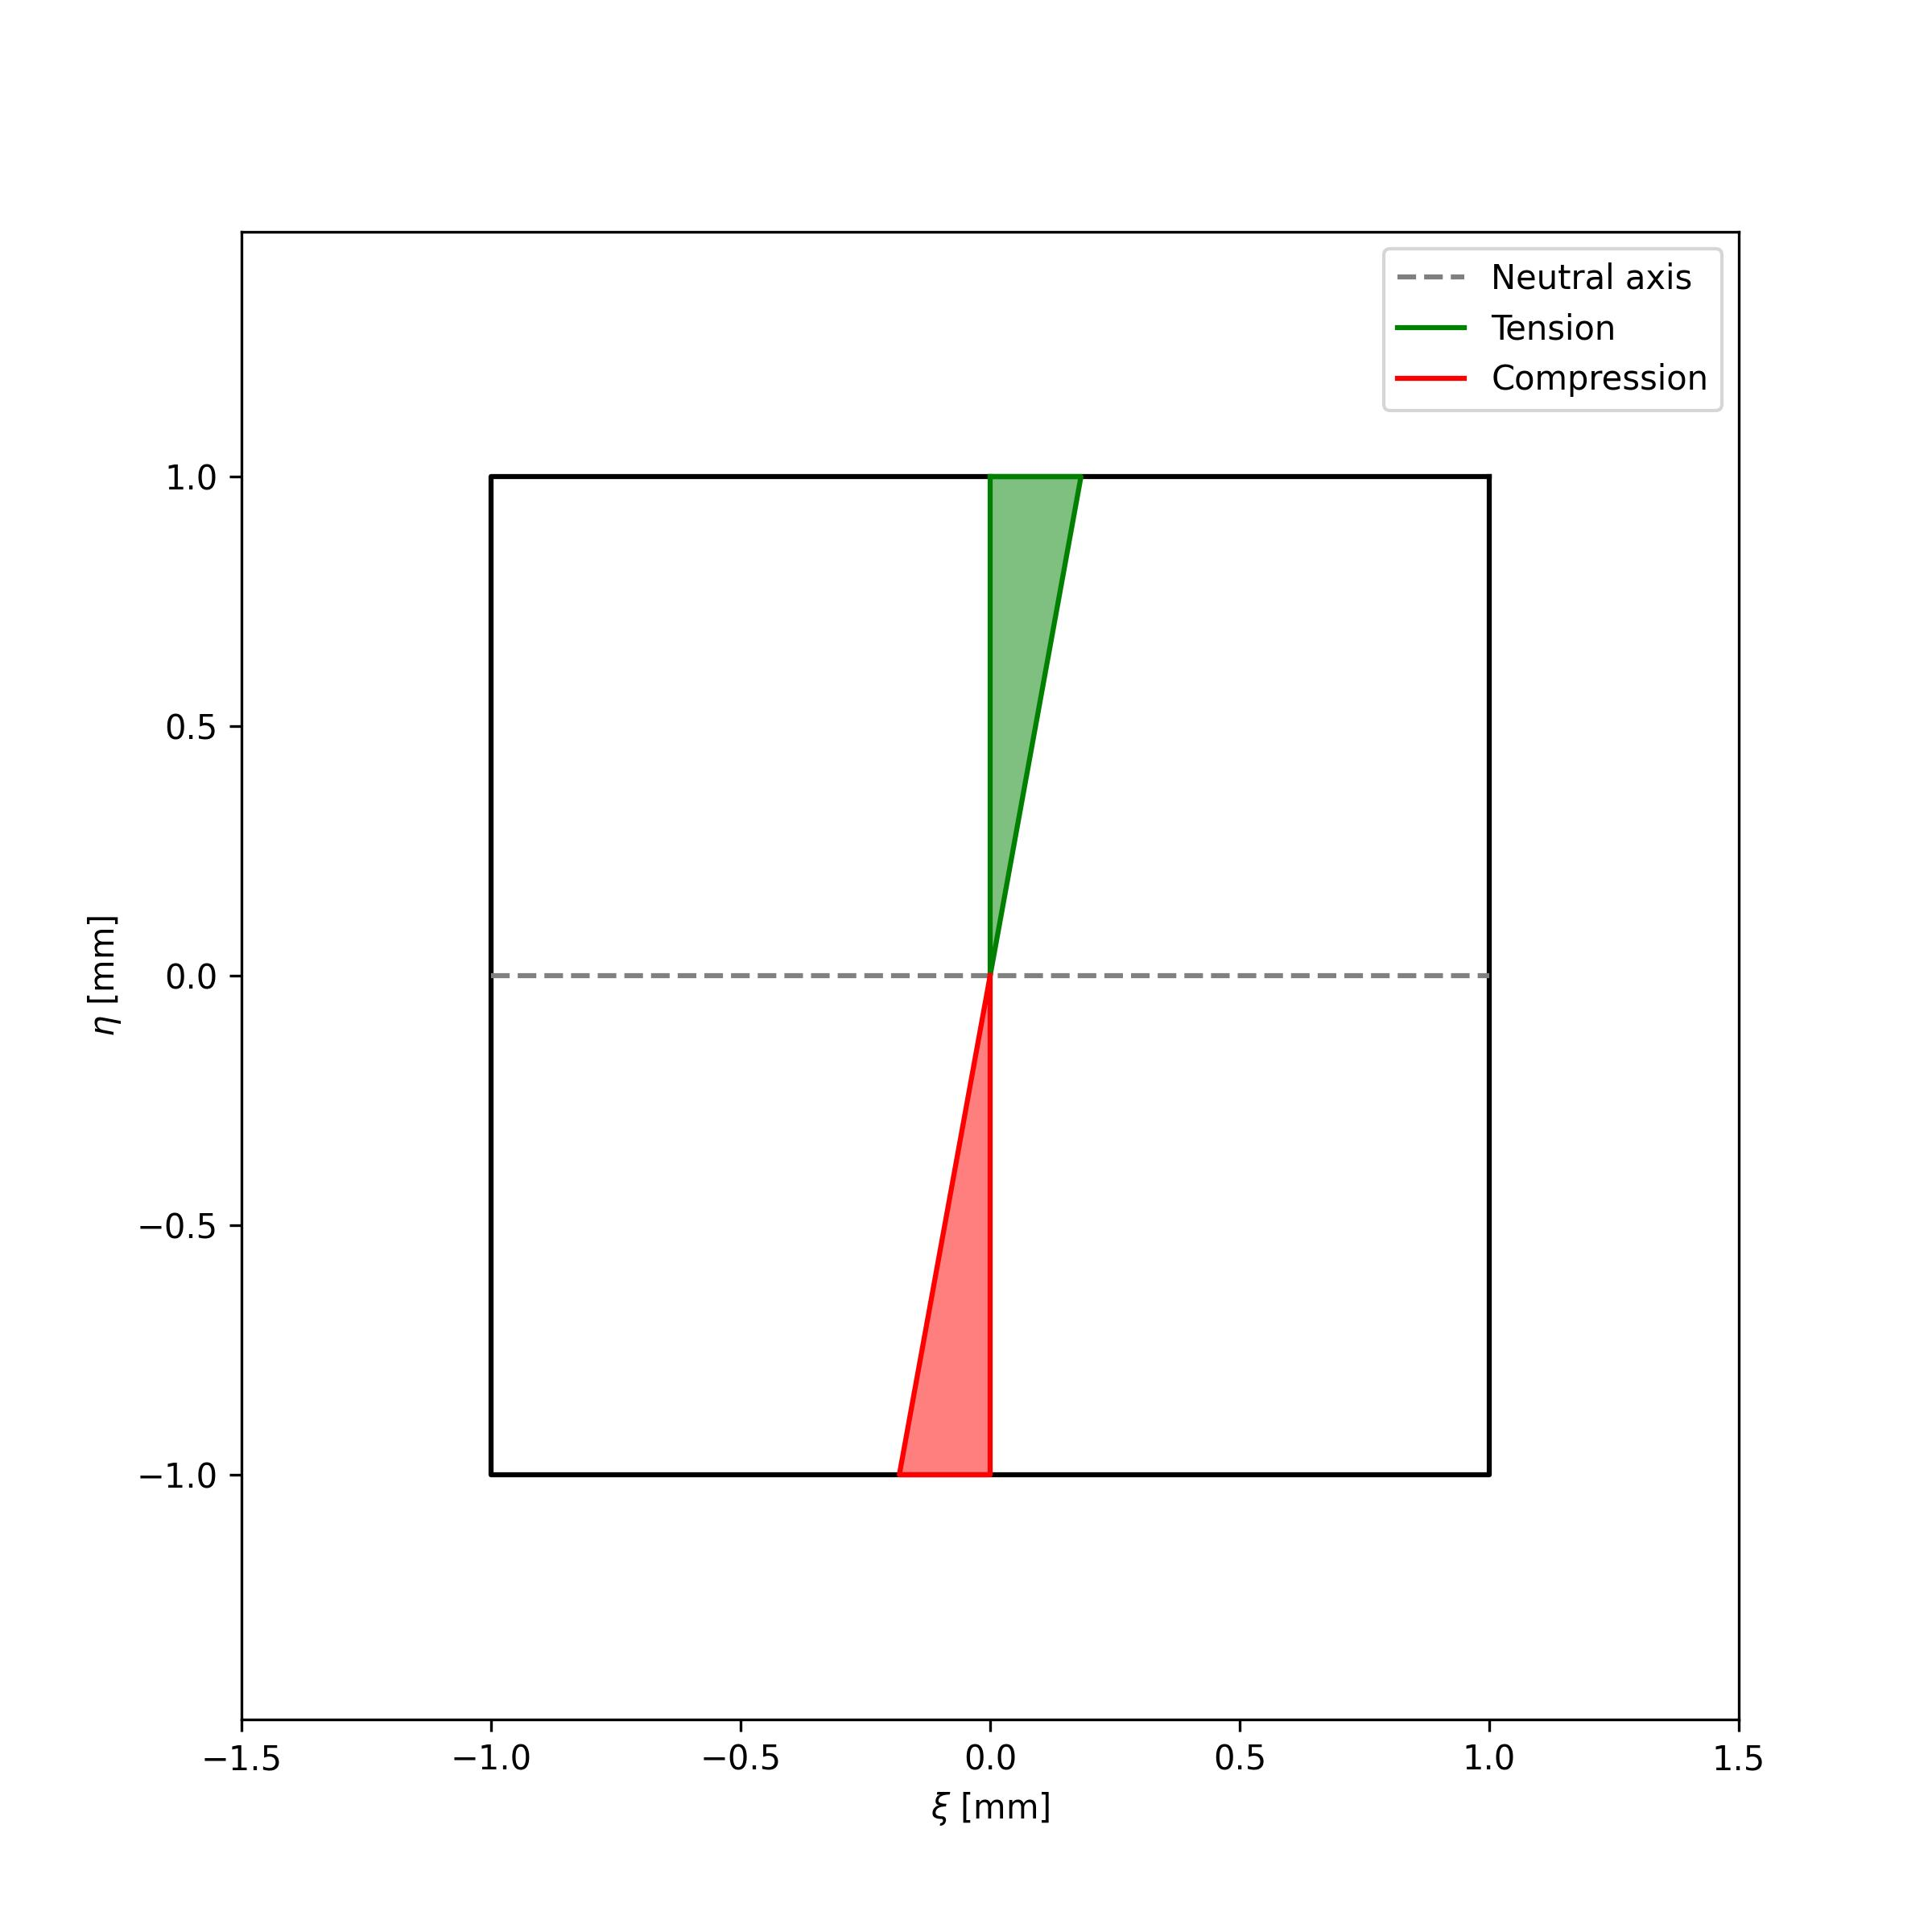
\includegraphics[width=0.8\textwidth]{Photos/p6.jpg}
	\caption{}
	\label{fig:strain}
\end{figure}
\item (\hyperref[code1]{Code, lines 198-211}) To plot the deformed position of the element, eq. 6.2-1 in \textit{Cook} is used. It state that,
\begin{align}
	\begin{Bmatrix} x \\ y \end{Bmatrix} = [N]\{c\} & \quad \text{and} \quad \begin{Bmatrix} u \\ v \end{Bmatrix} = [N]\{d\} \label{eq:621}
\end{align}
where $\{c\}$ contains the undeformed nodal coordinates in the physical space. Combining the two equations in (\ref{eq:621}) and applying the disruptive law for matrix manipulation, results in a equation that calculates the deformed coordinates in physical space as a function of $\xi$ and $\eta$. 
\begin{align}
	\begin{Bmatrix} x + u \\ y + v \end{Bmatrix} = [N]\{c\} + [N]\{d\} = [N]\{c+d\} \label{eq:deform}
\end{align} 

The undeformed and deformed states can be seen in figure (\ref{fig:defvsun}) below. 
\begin{figure}[H]
	\centering
	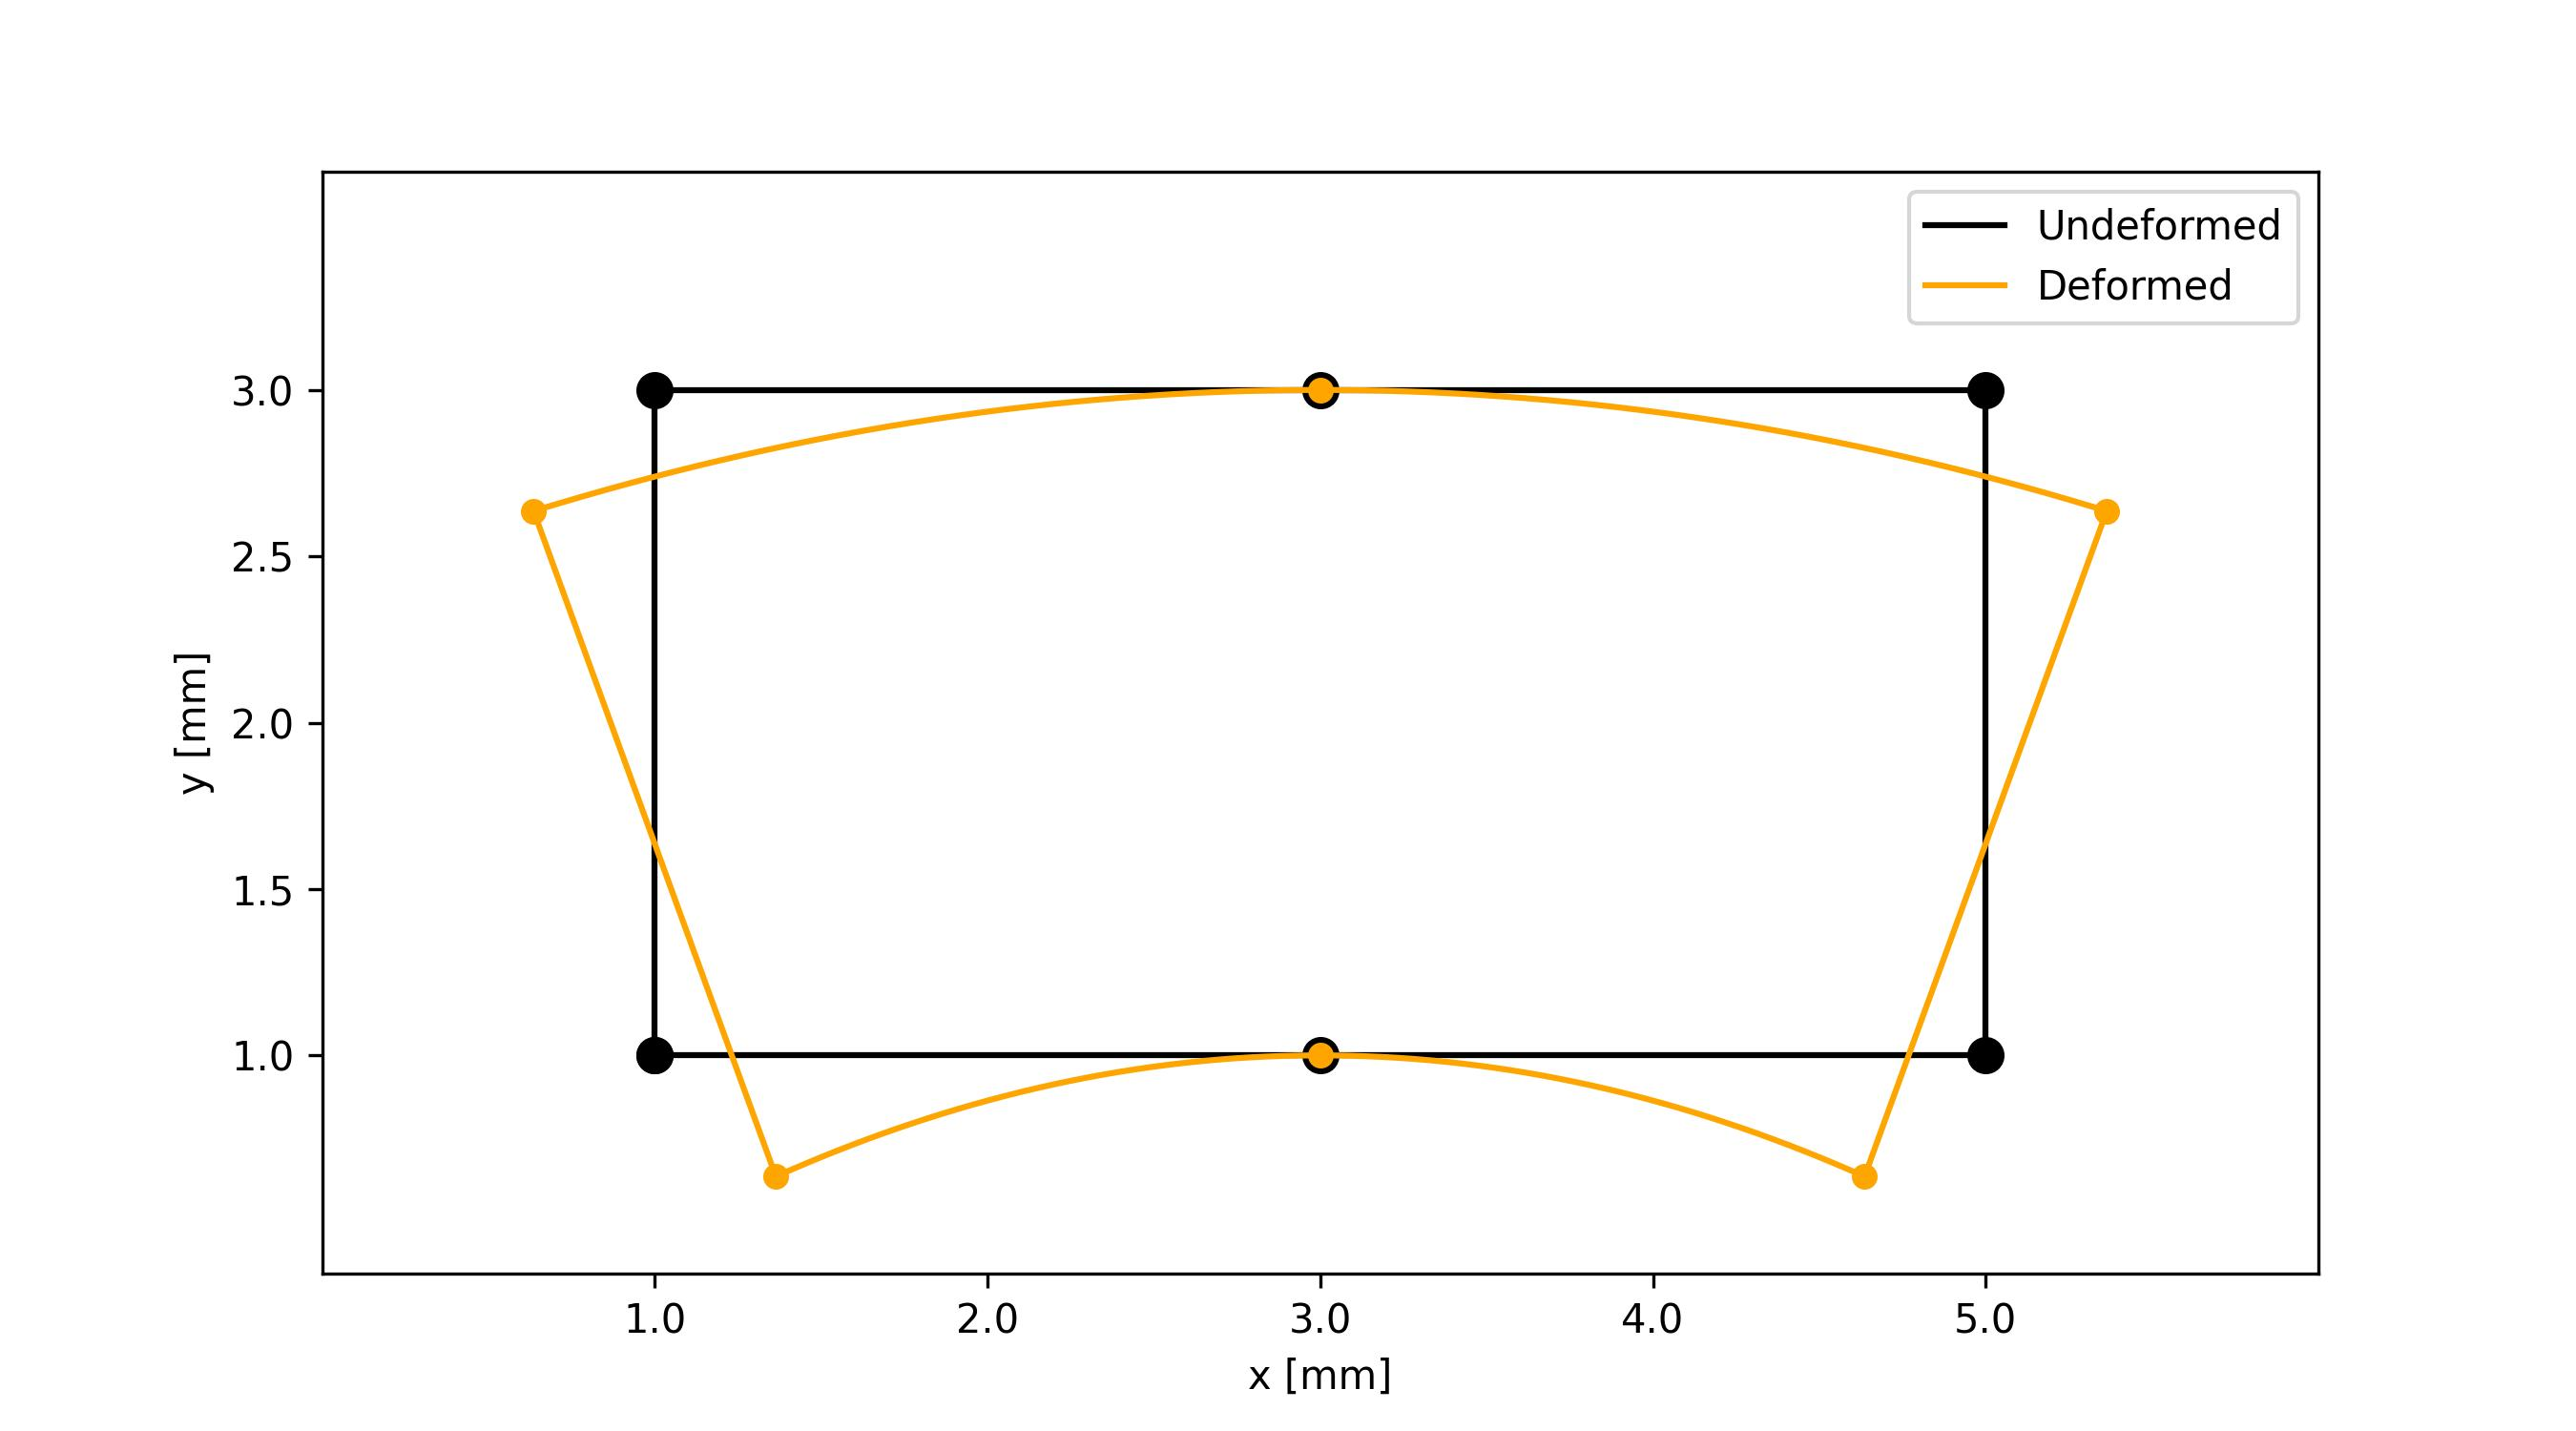
\includegraphics[width=0.8\textwidth]{Photos/p7.jpg}
	\caption{}
	\label{fig:defvsun}
\end{figure}


\end{enumerate}

(\hyperref[code1]{Code, lines 231-239}) The magnitude is calculated as 
\begin{align}
	\abs{u} = \sqrt{(x_f-x_i)^2 + (y_f-y_i)^2}
\end{align}
where $i$ is undeformed and $f$ is deformed. Figure (\ref{fig:magdist}) of the magnitude can be seen on the next page. 
\begin{figure}[H]
	\centering
	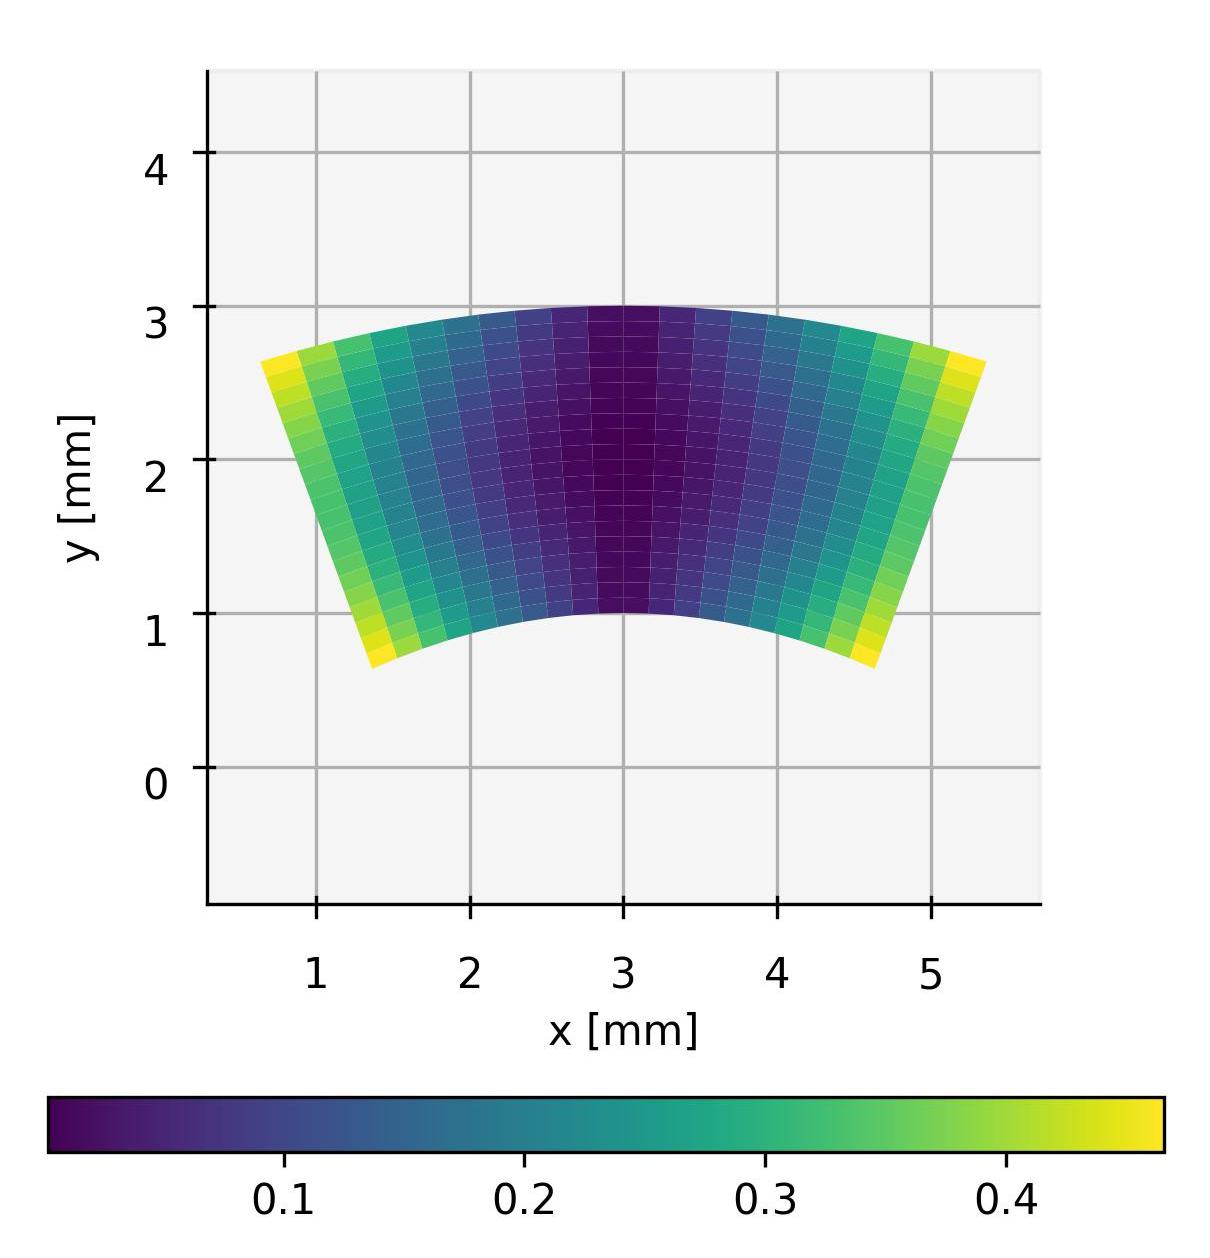
\includegraphics[width=0.8\textwidth]{Photos/p72.jpg}
	\caption{}
	\label{fig:magdist}
\end{figure}

\newpage
%%%%%%%%%%%%%%%%%%%%%%%%%%%%%%% Appendix %%%%%%%%%%%%%%%%%%%%%%%%%%%%%%%
\section*{Appendix}
\subsection*{Python Code} \label{code1}
\definecolor{bg}{rgb}{0.98,0.98,0.98}
\inputminted[bgcolor=bg, linenos, numbersep=5pt, frame=single, framesep=2mm]{Python}{Code/a2v22.py}

\end{document}

